% Control de avance del TPI, Etapa 1/2: especificacion del modelo conceptual.

\documentclass{article}

\usepackage{arxiv}

\usepackage[utf8]{inputenc} % allow utf-8 input
\usepackage[T1]{fontenc}    % use 8-bit T1 fonts
\usepackage[spanish]{babel}
\usepackage{hyperref}       % hyperlinks
\usepackage{url}            % simple URL typesetting
\usepackage{booktabs}       % professional-quality tables
\usepackage{amsfonts}       % blackboard math symbols
\usepackage{nicefrac}       % compact symbols for 1/2, etc.
\usepackage{microtype}      % microtypography
\usepackage{graphicx}
\usepackage{amsmath,amssymb}
\usepackage{float}
\usepackage{caption}
\usepackage{enumitem}
\usepackage{longtable}
\usepackage{array}

\graphicspath{{figuras/}}

\captionsetup{font=small,labelfont=bf,skip=6pt}

\renewcommand{\topfraction}{0.88}
\renewcommand{\bottomfraction}{0.70}
\renewcommand{\textfraction}{0.12}
\renewcommand{\floatpagefraction}{0.80}

\raggedbottom

\newcolumntype{L}[1]{>{\raggedright\arraybackslash}p{#1}}

\title{Especificación del modelo: evaluación mediante simulación del impacto de la
Línea F sobre la operación de la red de Subte de Buenos Aires \\[0.3ex]
\large Control de avance del TPI --- Etapa 1/2}

\author{
  \textbf{Bruno Neirotti}\textsuperscript{1} \qquad \textbf{Alexis Galasco}\textsuperscript{2} \qquad \textbf{Salami Tomás}\textsuperscript{3} \qquad \textbf{Mesapelle Giani}\textsuperscript{4} \qquad \textbf{Lovatti Francisco}\textsuperscript{5} \\[0.5ex]
  \textsuperscript{1}Legajo: 47792 -- \texttt{bneirotti@gmail.com} \\
  \textsuperscript{2}Legajo: 51474 -- \texttt{alexis.galasco123@gmail.com} \\
  \textsuperscript{3}Legajo: 51534 -- \texttt{tomas.salami1@gmail.com} \\
  \textsuperscript{4}Legajo: 52897 -- \texttt{gianimesapelle04@gmail.com} \\
  \textsuperscript{5}Legajo: 52420 -- \texttt{franciscolovatti08@gmail.com} \\[0.5ex]
  Universidad Tecnológica Nacional -- FRRo \\
  Grupo 3 \\
  Zeballos 1341, S2000, Argentina \\
}
\date{16 de septiembre de 2026}

\begin{document}
\maketitle

% ---------- Introducción ----------
\section{Introducción}

Este documento es la entrega previa al informe final del Trabajo Práctico Integrador
(Etapa 1/2, según la consigna publicada en el aula virtual de la materia): la
especificación del modelo conceptual sobre el que se va a construir el modelo de
simulación de eventos discretos en AnyLogic. No es el modelo en sí --- eso es la
Etapa 2/2, el informe final --- sino la descripción completa del sistema que ese
modelo va a representar: sus límites, sus componentes, sus datos y las preguntas que
tiene que poder contestar.

El sistema es la red de Subte de la Ciudad Autónoma de Buenos Aires, evaluada en dos
escenarios: la red actual (seis líneas) y la red con la incorporación de la futura
Línea F, un corredor de doce estaciones hoy en proceso de licitación. El criterio
central de esta entrega, según la consigna, es si la especificación está lo
suficientemente desarrollada como para que la siguiente etapa --- convertirla en un
modelo corriendo en AnyLogic --- no tenga que volver a definir ningún componente del
sistema.

Todo el contenido de este documento se apoya en el trabajo ya hecho del TPI: el
pipeline de datos (pasos 1 a 6 y 9 a 11, cerrado y verificado), las pruebas de
límites de AnyLogic PLE, y las decisiones de modelado registradas en
\texttt{decisiones.md}. No se repite acá la fundamentación completa de cada decisión;
se cita dónde encontrarla.

% ---------- 1. Sistema seleccionado ----------
\section{Sistema seleccionado}

La red de Subte de la Ciudad Autónoma de Buenos Aires: seis líneas en operación (A,
B, C, D, E, H), 90 nodos de línea-estación (78 complejos si se agrupan las estaciones
físicamente unidas por transbordo), operada por Subterráneos de Buenos Aires (SBASE).
Se modelan dos escenarios sobre el mismo sistema:

\begin{itemize}
  \item \textbf{Escenario base}: la red actual, sus seis líneas.
  \item \textbf{Escenario futuro}: la red actual más la \textbf{Línea F}, un corredor
    nuevo de 12 estaciones y 9,8~km entre Barracas y Palermo, hoy en licitación
    (proceso 10241-0094-LPU25), con inicio de servicio proyectado para 2031.
\end{itemize}

% ---------- 2. Descripción del problema ----------
\section{Descripción del problema}

La red es fuertemente radial: la mayoría de los viajes entre el sur y el norte de la
ciudad se resuelven transbordando en el macrocentro, lo que concentra la carga en
tramos y estaciones de combinación mientras otros sectores circulan holgados. La
Línea F se proyectó como corredor transversal para aliviar esa concentración, en
particular sobre la Línea C: el 70~\% de los viajes que incluyen una etapa en la C
combinan con el ferrocarril Roca, que la Línea F también vincula.

El problema es que \textbf{no existe, en ninguna fuente pública ni en el expediente
oficial del proyecto, una evaluación del efecto de la Línea F sobre el conjunto de la
red}. El Estudio de Impacto Ambiental dimensiona la línea nueva y publica su perfil
de demanda propio, pero no compara el funcionamiento de la red con y sin el
proyecto, no publica una matriz origen--destino de la red completa, y no dice qué
frecuencia de servicio haría falta para lograr el alivio que se anuncia. El TPI
construye esa evaluación: un modelo de simulación de eventos discretos de la red
actual, calibrado con datos públicos, al que se le agrega la Línea F para medir la
diferencia.

% ---------- 3. Límites del sistema ----------
\section{Límites del sistema}

\textbf{Dentro del sistema:}
\begin{itemize}
  \item Las seis líneas actuales, sus 90 nodos (par línea-estación) y sus
    194 aristas (166 tramos, 28 transbordos), con calibración a dos velocidades (ver
    más abajo).
  \item En el escenario futuro, la Línea F completa (traza única, sin habilitación
    parcial).
  \item La demanda de pasajeros que entra al sistema por cualquier estación, su
    elección de ruta, su espera en andén, su viaje a bordo, sus transbordos y su
    salida por la estación de destino.
  \item El despacho de formaciones desde cada cabecera y su circulación por la línea.
\end{itemize}

\textbf{Fuera del sistema:}
\begin{itemize}
  \item El Premetro.
  \item Los ferrocarriles Roca y San Martín y el transporte de superficie: son fuente
    de parte de la demanda de transferencia en los nodos de combinación (p.~ej.
    Constitución), pero su operación no se simula. Entran como generador exógeno de
    pasajeros, no como subsistema modelado.
  \item La obra civil y las etapas constructivas de la Línea F: el modelo simula la
    operación de la línea terminada, no la construcción.
  \item Los accesos peatonales fuera de la red (calles, veredas): la caminata que se
    modela es solo la interna a cada complejo de estación (transbordo).
\end{itemize}

\textbf{Profundidad diferenciada.} El corredor de la Línea F y las líneas con las
que combina (A, C, D, H) se calibran y validan a fondo; el resto de la red (B, E, y
los tramos de A/C/D/H sin combinación con la F) se representa con verificación
agregada (totales, reparto por línea) pero sin el mismo nivel de ajuste tramo a
tramo. Decidido con el grupo el 16/09/2026.

\textbf{Horizonte temporal.} Un día hábil típico completo, servicio de punta a
punta (\raise.17ex\hbox{$\scriptstyle\sim$}19~horas), excluyendo sábados, domingos,
feriados y los días atípicos identificados en el pipeline (25 días hábiles con
anomalías, el 10/04/2025 de paro general, marzo de 2025 sin datos de despachos).

% ---------- 4. Entidades ----------
\section{Entidades}

\begin{table}[H]
\centering
\small
\begin{tabular}{@{}L{2.6cm}L{4.5cm}L{7cm}@{}}
\toprule
Entidad & Qué es & Atributos principales \\
\midrule
Pasajero & La entidad dinámica principal. Un agente = un pasajero. & Complejo de
  origen, complejo de destino, hora de generación, ruta asignada (secuencia de
  nodos), línea(s) de ascenso y descenso, estado actual. \\
Formación & Tren que circula por una línea, despachado desde una cabecera. & Línea,
  sentido, cantidad de coches, capacidad total, hora de despacho, posición en la
  red. \\
\bottomrule
\end{tabular}
\caption{Entidades del modelo.}
\end{table}

Los \textbf{nodos} (par línea-estación) y \textbf{complejos} (estación física) no son
entidades que fluyen por el sistema, sino la topología fija sobre la que se mueven
las entidades (ver sección~\ref{sec:relaciones}).

% ---------- 5. Recursos ----------
\section{Recursos}

\begin{table}[H]
\centering
\small
\begin{tabular}{@{}L{3.2cm}L{5cm}L{5.5cm}@{}}
\toprule
Recurso & Qué limita & Capacidad \\
\midrule
Capacidad de coche de una formación & Cuántos pasajeros aborda una formación en un
  tramo & Coches por formación (medido, por línea) $\times$ capacidad por coche
  (supuesto, sección~\ref{sec:supuestos}) \\
Andén & Espacio donde se acumulan los pasajeros que esperan o transbordan & Sin tope
  físico modelado por ahora; se mide la ocupación para reportar aglomeración, no se
  restringe el ingreso \\
\bottomrule
\end{tabular}
\caption{Recursos del modelo.}
\end{table}

El pasajero \textbf{seiza} la capacidad de una formación al abordar en un tramo y la
\textbf{libera} al bajar (sea por transbordo o por llegar a destino). Si la
formación llega llena, el pasajero no aborda y queda en el andén para el próximo
evento de llegada de formación en esa línea y sentido (ver
sección~\ref{sec:supuestos}).

% ---------- 6. Procesos ----------
\section{Procesos}

\textbf{Proceso del pasajero:}
\begin{enumerate}
  \item Generación en un complejo, según la tasa de la hora y el reparto
    intrahorario.
  \item Asignación de ruta: se lee de la tabla de caminos mínimos, precalculada
    fuera del modelo (Dijkstra con penalización de transbordo, ya resuelto en el
    pipeline). No hay asignación dinámica dentro de la simulación.
  \item Acceso al andén de ascenso (tiempo cero dentro del complejo de origen).
  \item Espera en andén hasta la llegada de una formación de la línea/sentido que
    corresponde.
  \item Intento de embarque: si hay capacidad disponible, aborda; si no, permanece
    en andén esperando la próxima formación.
  \item Viaje a bordo: recorre uno o más tramos con el tiempo de cada uno (tiempo de
    tramo más detención endógena).
  \item En cada nodo de la ruta: decide si baja (transbordo o destino) o continúa a
    bordo, según la ruta ya asignada.
  \item Si transborda: caminata interna al complejo (tiempo mínimo de combinación
    del GTFS como piso) y vuelve al paso 4 para la línea siguiente.
  \item Si llega a destino: sale del sistema.
\end{enumerate}

\textbf{Proceso de la formación:}
\begin{enumerate}
  \item Despacho desde una cabecera, con intervalo tomado de la distribución
    empírica medida por línea, cabecera y hora (líneas actuales) o de la variable
    de escenario de intervalo entre trenes (Línea F, ver
    sección~\ref{sec:variables}). En la apertura del servicio (5:30) las
    formaciones arrancan desde las estaciones intermedias donde lo hacen en la
    operación real, medidas en el dataset de despachos.
  \item Recorrido tramo a tramo: tiempo de viaje más detención en cada estación
    intermedia (mínimo de diseño 24~s para las líneas actuales, 30~s para la Línea
    F, endógeno según ascensos/descensos).
  \item En cada estación: descenso de los pasajeros que bajan ahí, ascenso de los
    que esperan en andén hasta llenar la capacidad disponible.
  \item Llegada a la cabecera opuesta: la formación se recicla al \textit{pool}
    (arquitectura de \textit{pool} declarado y reciclado) y queda disponible para
    un nuevo despacho.
\end{enumerate}

% ---------- 7. Colas ----------
\section{Colas}

\begin{table}[H]
\centering
\small
\begin{tabular}{@{}L{4.5cm}L{4.5cm}L{4.5cm}@{}}
\toprule
Cola & Dónde & Disciplina \\
\midrule
Pasajeros esperando abordar & En cada andén, por complejo, línea y sentido & FIFO
  dentro de cada llegada de formación; se agregan los que no lograron subir en la
  formación anterior \\
Pasajeros en transbordo & Caminando dentro de un complejo, entre el andén de
  descenso y el de ascenso de la línea siguiente & No es cola de espera por
  recurso, es un retardo de tiempo fijo (piso del GTFS) \\
\bottomrule
\end{tabular}
\caption{Colas del modelo.}
\end{table}

No hay cola de formaciones: se despachan según la distribución de intervalos, no
esperan un recurso compartido para salir de cabecera.

% ---------- 8. Variables ----------
\section{Variables}
\label{sec:variables}

\textbf{Variables de estado} (cambian durante la corrida, se leen para calcular
indicadores):
\begin{itemize}
  \item Cantidad de pasajeros esperando en cada andén (por complejo, línea,
    sentido).
  \item Ocupación de cada formación en circulación.
  \item Cantidad de formaciones circulando por línea en un instante dado.
  \item Contador acumulado de pasajeros que no lograron abordar en el primer
    intento.
\end{itemize}

\textbf{Variables de decisión / de escenario} (se fijan antes de cada corrida y se
recorren en el análisis de sensibilidad):
\begin{itemize}
  \item Intervalo entre trenes de la Línea F, entre 90 y 189~s.
  \item Detención de la Línea F, con piso de 30~s.
  \item Criterio de reparto de demanda fuera de las horas pico (perfil por par,
    perfil de red, o perfil por complejo de origen).
\end{itemize}

% ---------- 9. Parámetros ----------
\section{Parámetros}
\label{sec:parametros}

Se listan en detalle en \texttt{docs/guia-del-modelo.md}, sección 4. Resumen por
categoría:

\begin{itemize}
  \item \textbf{Fijos} (dato medido o de diseño oficial): topología (90 nodos, 166
    tramos, 28 transbordos), tiempo y distancia de cada tramo (GTFS), demanda por
    par y hora (SBASE más el paso 5 del pipeline), ruta de cada par, intervalos de
    despacho de las líneas actuales, coches por formación, y los parámetros
    oficiales de la Línea F (distancias, capacidad de 1.075~pasajeros por
    formación, velocidades 90/70/45~km/h, aceleración 1~m/s\textsuperscript{2},
    frenado 1,1~m/s\textsuperscript{2}, flota de 25 formaciones).
  \item \textbf{Calibrado}: penalización por transbordo, 120~s.
  \item \textbf{Variable de escenario}: ver sección~\ref{sec:variables}.
  \item \textbf{Supuesto}: capacidad por coche de las líneas actuales,
    comportamiento del pasajero que no aborda (sección~\ref{sec:supuestos}).
\end{itemize}

% ---------- 10. Eventos ----------
\section{Eventos}

\begin{table}[H]
\centering
\small
\begin{tabular}{@{}L{5.5cm}L{8cm}@{}}
\toprule
Evento & Dispara \\
\midrule
Generación de un pasajero & Entra a la cola del andén de su complejo de origen \\
Llegada de una formación a una estación & Descenso de pasajeros, luego ascenso hasta
  capacidad \\
Partida de una formación de una estación & Fin de la detención, la formación pasa
  al siguiente tramo \\
Pasajero completa un transbordo & Se reincorpora a la cola de andén de la línea
  siguiente \\
Pasajero llega a destino & Sale del sistema, se registra el tiempo total de viaje \\
Formación llega a cabecera & Se recicla al \textit{pool}, disponible para nuevo
  despacho \\
Cambio de franja horaria & Cambia la tasa de generación de pasajeros \\
Fin del período de calentamiento & Empiezan a contar los indicadores de la corrida \\
Fin de la corrida (día completo) & Se cierra la réplica; conservación de entidades:
  ingresados = arribados + a bordo + en andén al corte \\
\bottomrule
\end{tabular}
\caption{Eventos del modelo.}
\end{table}

% ---------- 11. Estados ----------
\section{Estados}

\textbf{Estado del pasajero} (máquina de estados simple): generado
$\rightarrow$ esperando en andén $\rightarrow$ a bordo $\rightarrow$
(transbordando $\rightarrow$ esperando en andén $\rightarrow$ a bordo)$^{*}$
$\rightarrow$ arribado.

\textbf{Estado de la formación}: en cabecera (esperando despacho) $\rightarrow$ en
tránsito (entre estaciones) $\rightarrow$ detenida (en estación) $\rightarrow$ en
cabecera opuesta (reciclada).

\textbf{Estado del sistema} en un instante dado: el vector completo de pasajeros
esperando por andén, pasajeros a bordo por formación y formaciones en circulación
por línea. Es lo que el motor de eventos discretos actualiza en cada evento.

% ---------- 12. Relaciones entre componentes ----------
\section{Relaciones entre componentes}
\label{sec:relaciones}

\begin{itemize}
  \item La topología es un \textbf{grafo dirigido}: nodos = par línea-estación (90),
    aristas = tramo (166) o transbordo (28). Alberti y Pasco obligan a que sea
    dirigido: se sirven en un solo sentido cada una.
  \item Los 90 nodos se agrupan en \textbf{78 complejos} (componentes conexas del
    grafo de transbordos): un complejo es donde el pasajero entra y sale del
    sistema; el nodo es por donde circula el tren.
  \item El pasajero \textbf{usa} la capacidad de la formación mientras está a bordo
    de un tramo (relación de recurso compartido).
  \item El andén \textbf{conecta} la demanda que llega caminando (generación o
    transbordo) con las formaciones que llegan circulando.
  \item El transbordo \textbf{conecta} dos líneas dentro de un mismo complejo;
    caminar dentro del complejo de origen o destino no cuenta como transbordo (vale
    cero).
  \item En el escenario futuro, la Línea F se \textbf{agrega} como nodos y aristas
    nuevos, conectados a la red existente en las estaciones de combinación (seis
    declaradas por el Estudio de Impacto Ambiental, dos adicionales solo en el mapa
    oficial). Se recalcula la tabla de caminos mínimos con el mismo procedimiento:
    la redistribución de pasajeros es resultado del cambio de topología, no un
    supuesto impuesto línea por línea. El reparto que resulte se contrasta después
    contra las matrices origen-destino de SBASE~2019 en los nodos de combinación
    (ver sección~\ref{sec:supuestos} y \texttt{decisiones.md}), nunca al revés.
\end{itemize}

% ---------- 13. Datos de entrada ----------
\section{Datos de entrada}

Los cinco archivos que el pipeline de datos deja listos, todos en
\texttt{data/processed/}:

\begin{table}[H]
\centering
\small
\begin{tabular}{@{}L{5.3cm}L{8.2cm}@{}}
\toprule
Archivo & Qué aporta al modelo \\
\midrule
\texttt{grafo\_nodos.csv} & Los 90 nodos con sus atributos \\
\texttt{grafo\_aristas.csv} & Los 194 tramos/transbordos con tiempos y distancias \\
\texttt{caminos\_minimos.csv} & La ruta de cada uno de los 6.006 pares ordenados \\
\texttt{demanda\_modelo\_\allowbreak od\_hora.csv} & 827.289 viajes por día, 71.686 celdas de
  (par, hora) \\
\texttt{demanda\_modelo\_\allowbreak intrahorario.csv} & Reparto de cada hora en bloques de
  15~minutos \\
\bottomrule
\end{tabular}
\caption{Insumos de datos que consume el modelo.}
\end{table}

A eso se suman, para el modelo en AnyLogic:
\begin{itemize}
  \item \textbf{Distribuciones de intervalos de despacho}: sobre 319.792
    intervalos medidos entre julio y diciembre de 2025 se hizo el procedimiento de la materia (histogramas, máxima
    verosimilitud de cinco familias y bondad de ajuste). La lognormal gana en la
    mayoría de las celdas, pero la Línea H es bimodal y ninguna familia teórica la
    reproduce, así que el modelo usa la \textbf{distribución empírica} en todas.
    Se excluyen los cortes de servicio sin causa registrada.
  \item \textbf{Distribución de llegada de pasajeros}, derivada de la tasa horaria e
    intrahoraria (no homogénea).
  \item \textbf{Parámetros de la Línea F}, tomados directamente del expediente
    oficial (sección~\ref{sec:parametros}).
\end{itemize}

% ---------- 14. Indicadores de desempeño ----------
\section{Indicadores de desempeño}

\begin{table}[H]
\centering
\small
\begin{tabular}{@{}L{5.5cm}L{8cm}@{}}
\toprule
Indicador & ¿Tiene contraparte observable? \\
\midrule
Ocupación a bordo por tramo & Sí, contra el perfil de carga de SBASE (dos horas
  pico, 2024, con ajuste declarado por SBASE) \\
Reparto de ascensos por línea en combinaciones & Sí, parcial, contra molinetes y la
  línea de ascenso declarada \\
Tasa de transbordo & Sí, contra el observado (1,371 en la mañana, 1,426 en la
  tarde) \\
Concentración horaria & Sí, 9,9~\% medido sobre molinetes \\
Tiempo de viaje puerta a puerta & Es salida directa del modelo; se compara entre
  escenarios, no hay observado de referencia \\
Tiempo de espera en andén & Salida del modelo, sin observado de referencia \\
Aglomeración de andén & No, ninguna fuente la registra \\
Pasajeros que no logran abordar & No, depende del supuesto de comportamiento \\
Detención real (líneas actuales) & No, solo hay piso de diseño (24~s) \\
\bottomrule
\end{tabular}
\caption{Indicadores de desempeño y su validabilidad.}
\end{table}

Todos se reportan \textbf{comparados entre escenarios} (red actual contra red con
Línea F, y por variante de intervalo entre trenes de la Línea F), con un mínimo de
diez replicaciones por escenario, descartando el período de calentamiento e
informando intervalos de confianza.

% ---------- 15. Supuestos ----------
\section{Supuestos}
\label{sec:supuestos}

\begin{itemize}
  \item \textbf{Capacidad por coche de las líneas actuales}: no hay dato oficial;
    se toma de referencia la capacidad por coche de la Línea F (1.075 pasajeros
    entre 6 coches, unos 179 por coche), aclarando que para las líneas de 5 coches
    es una extrapolación.
  \item \textbf{Detención de las líneas actuales}: endógena (según ascensos y
    descensos), con piso de 24~s de diseño del GTFS. El modelo se verifica primero
    con la detención fija en ese piso, y el término por pasajero se agrega en la
    calibración, con su coeficiente como supuesto declarado.
  \item \textbf{Comportamiento del pasajero que no aborda}: espera la próxima
    formación de la misma línea y sentido en el mismo andén; no cambia de ruta ni
    abandona el sistema. Regla declarada, no medida, confirmada por el grupo el
    21/09/2026.
  \item \textbf{Caminata de transbordo}: se usa el tiempo mínimo de combinación del
    GTFS como piso; no es una caminata cronometrada.
  \item \textbf{Sentido 1 de la Línea E}: en el GTFS publicado, sus distancias son
    copia de las del sentido 0 y sus tiempos no se corresponden con ellas. Se toman
    los tiempos del sentido 0, que es lo que hacen las otras cinco líneas del mismo
    archivo. Afecta al 1,0~\% de los caminos.
  \item \textbf{Etapas marcadas como incompletas} (4,1~\%): se conservan. Solo
    entran en la forma de la curva horaria fuera de las horas pico, no en el nivel
    de la demanda; medido, excluirlas cambia de hora el 1,33~\% de los viajes del
    día.
  \item \textbf{Asignación de ruta todo-o-nada}: cada par origen-destino manda todo
    su flujo por un único camino precalculado; no se reparte entre alternativas
    cercanas en tiempo.
  \item \textbf{Demanda del modelo}: la matriz de SBASE (diaria más horas pico) como
    base, con el resto del día desagregado según el perfil del dataset de viajes y
    etapas (supuesto propio, sujeto a análisis de sensibilidad).
  \item \textbf{Penalización de transbordo fija en 120~s}: el dato no identifica el
    parámetro por encima de 30~s; 120~s se sostiene por argumento físico.
  \item \textbf{Profundidad de calibración diferenciada}: corredor Línea F más
    A/C/D/H a fondo, B y E con verificación agregada.
  \item \textbf{Intervalo entre trenes de la Línea F como variable de escenario, no
    como dato fijo}: la fuente oficial dice explícitamente que el plan de servicio
    no existe.
  \item \textbf{Demanda futura de la Línea F}: no hay medición posible; la nota
    técnica \textit{Análisis de Demanda Línea F} (SBASE, 2019) --- obtenida en
    fuente primaria por la solicitud N.\textsuperscript{o}~00934682/26, no solo
    citada por el EsIA --- se usa \textbf{solo como contraste, nunca como insumo del
    modelo} (decidido el 16/09/2026, ver \texttt{decisiones.md}), con tres
    salvedades: implica una concentración horaria (\textasciitilde 25~\% de la
    demanda diaria en la hora pico) que la red actual no exhibe (9,9~\%); su cuadro
    de intervalos de entrada para las líneas actuales es un supuesto de mejora de
    frecuencia de 2019 que no se concretó (los despachos medidos de 2025 son más
    espaciados en las seis líneas); y su trazado tiene \textbf{13 estaciones con
    terminal sur en California}, no las 12 vigentes con terminal en Brandsen, así
    que la correspondencia estación por estación con el diseño actual debe
    verificarse por geometría antes de comparar, no darse por sentada.
\end{itemize}

% ---------- 16. Preguntas de simulación ----------
\section{Preguntas de simulación}

\begin{enumerate}
  \item ¿Qué tan bien reproduce el modelo, en el escenario base, la ocupación a
    bordo por tramo y el reparto de ascensos por línea que mide SBASE en hora
    pico? (Verificación del modelo antes de comparar escenarios.)
  \item ¿Cómo cambian la ocupación de coche, la aglomeración de andén, el tiempo de
    viaje y la tasa de transbordo al incorporar la Línea F con su traza completa,
    frente al escenario base?
  \item Dentro del rango de intervalo entre trenes de 90 a 189~s, ¿qué frecuencia de
    la Línea F es necesaria para lograr un alivio medible en la Línea C y en el
    corredor de combinación, y a partir de qué punto los indicadores dejan de
    mejorar de forma apreciable?
  \item ¿Cómo se redistribuye la demanda entre las seis líneas existentes y la
    Línea F (cambios en el reparto por línea, en la tasa de transbordo y en los
    tiempos de viaje agregados de la red)?
  \item ¿Qué tan sensibles son los indicadores centrales a los supuestos propios del
    trabajo: la desagregación temporal fuera de las horas pico, el coeficiente de
    detención por pasajero, y la regla de comportamiento del pasajero que no
    aborda?
\end{enumerate}

% ---------- 17. Diagrama conceptual final ----------
\section{Diagrama conceptual final}

La figura~\ref{fig:diagrama-conceptual} muestra, en dos carriles paralelos
sincronizados por el recurso compartido (capacidad de coche), el flujo del pasajero
y el de la formación descriptos en la sección~6, con los lazos de espera y
transbordo, y una marca visual sobre el despacho de la Línea F señalando el
intervalo entre trenes como variable de escenario. Se generó con la herramienta de
diagramación \textit{archify}; la fuente editable queda en
\texttt{docs/figuras/} del repositorio.

\begin{figure}[H]
  \centering
  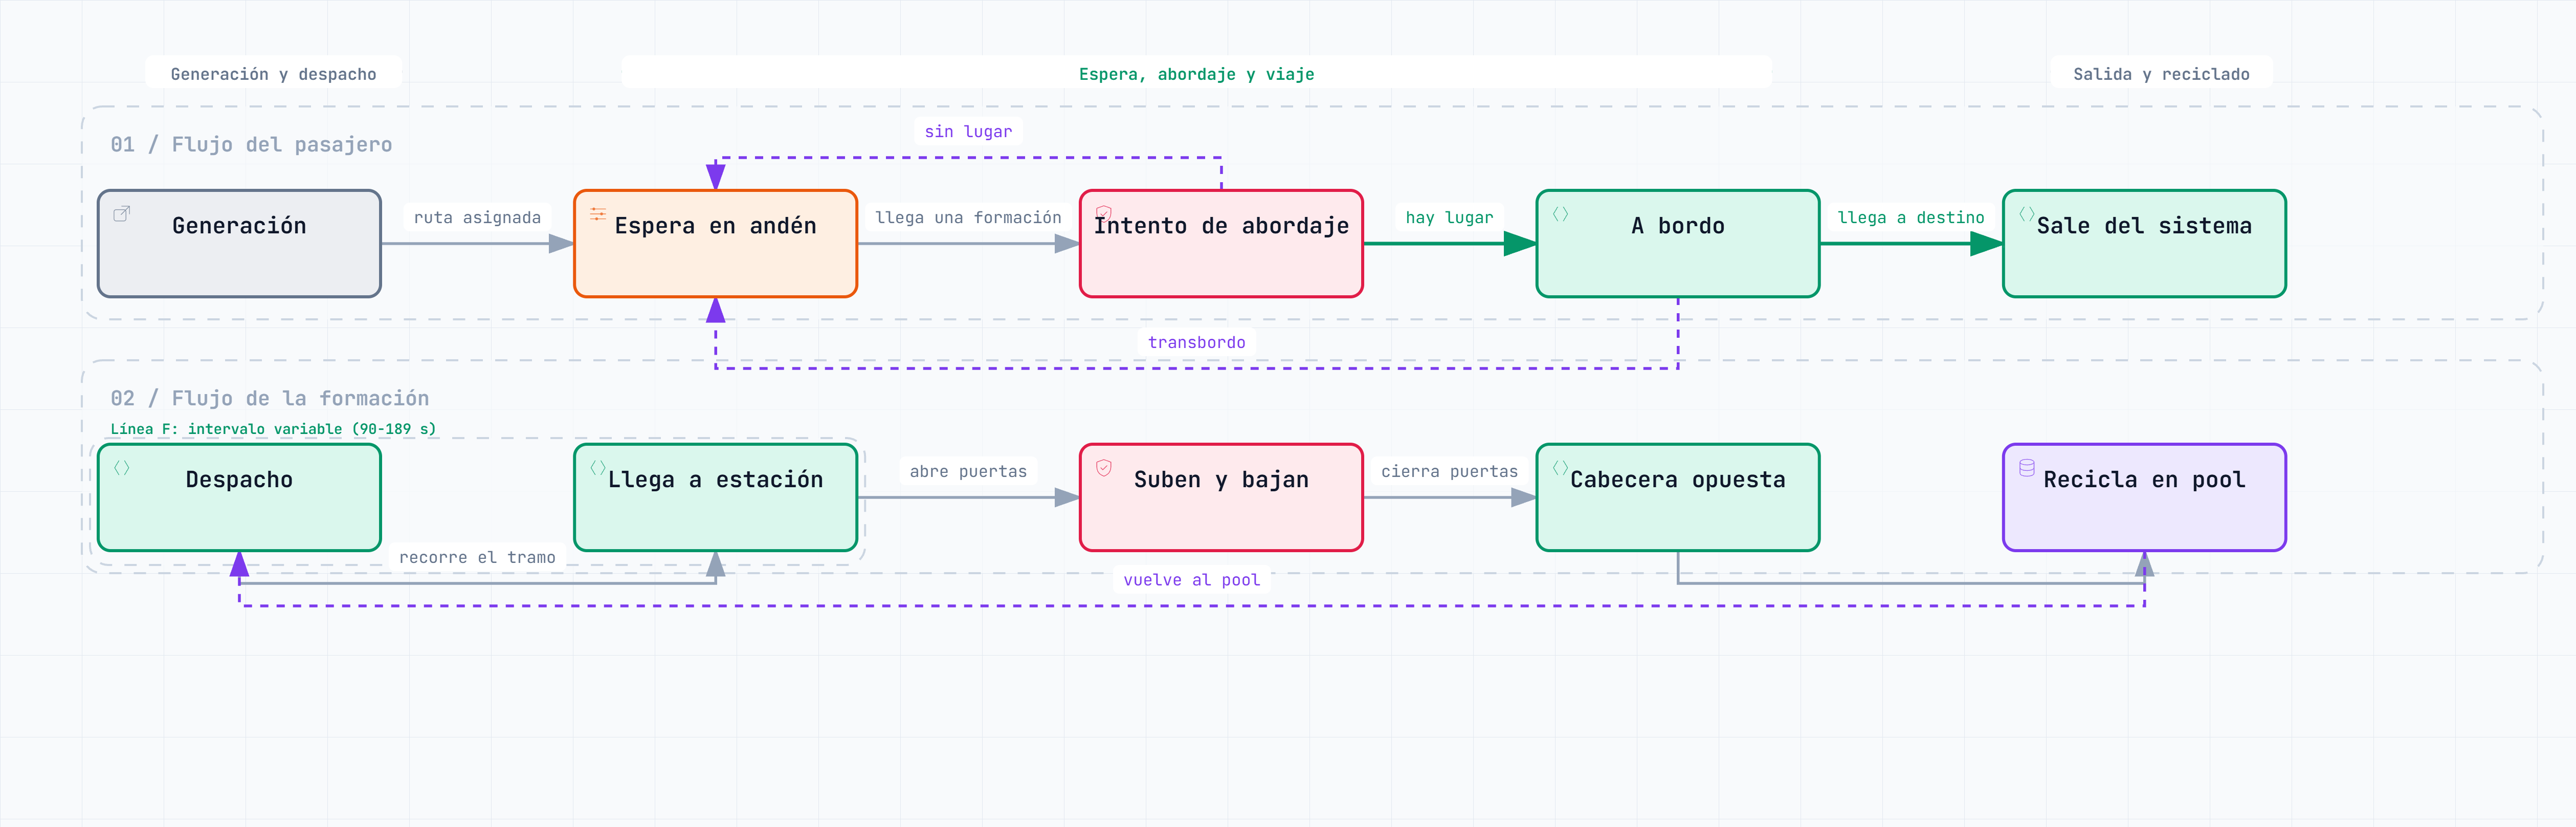
\includegraphics[width=\linewidth]{diagrama-conceptual-modelo.png}
  \caption{Modelo conceptual del pasajero y de la formación, con el recurso
  compartido y los dos escenarios evaluados.}
  \label{fig:diagrama-conceptual}
\end{figure}

% ---------- Glosario ----------
\section*{Glosario}
\addcontentsline{toc}{section}{Glosario}

Términos propios del proyecto y del dominio de simulación que aparecen en este
documento. Se prefiere el término en español cuando existe uno claro y ya usado por
las fuentes oficiales del proyecto; se mantienen en inglés los nombres propios de
bloques de software y los tecnicismos sin traducción establecida.

\begin{description}[leftmargin=3.2cm, style=nextline]
  \item[Complejo] Agrupación de nodos de distintas líneas unidos por un transbordo
    peatonal interno (p.~ej. Constitución~C y Constitución~E son un mismo
    complejo). Es la unidad de la demanda y de las rutas.
  \item[Nodo] Par línea-estación. Es la unidad de la topología física por la que
    circulan los trenes; no coincide uno a uno con el complejo.
  \item[Intervalo entre trenes] Tiempo entre dos despachos sucesivos de una misma
    línea y sentido. Se prefiere a ``headway'' porque es el término que usan el
    Estudio de Impacto Ambiental y el pliego de licitación de la Línea F.
  \item[Penalización por transbordo] Costo de tiempo adicional, calibrado en 120~s,
    que se suma al tiempo de viaje real para elegir la ruta de cada par
    origen-destino; representa la espera y el desagrado del cambio de línea.
  \item[Asignación todo-o-nada] Criterio de ruteo en el que cada par
    origen-destino manda el 100~\% de su demanda por un único camino, sin repartir
    entre alternativas.
  \item[\textit{Pool}] Arquitectura de AnyLogic en la que los agentes (formaciones)
    se reciclan y reingresan al sistema en lugar de generarse y destruirse en cada
    ciclo. Se mantiene en inglés por ser terminología estándar de la biblioteca de
    simulación.
  \item[\texttt{Enter} / \texttt{Exit}] Bloques de AnyLogic usados para reciclar
    agentes desde un \textit{pool}, en lugar de \texttt{Source}/\texttt{Sink} (que
    crean y destruyen agentes). Nombres propios de la herramienta, no se traducen.
  \item[PML] \textit{Process Modeling Library}, la biblioteca de AnyLogic elegida
    para el modelo por estar exenta del tope de 5~horas simuladas de la licencia
    PLE.
  \item[GTFS] \textit{General Transit Feed Specification}, formato estándar de
    datos de transporte público del que sale la topología y los tiempos de tramo de
    la red. Nombre propio del formato, no se traduce.
  \item[EsIA] Estudio de Impacto Ambiental del proyecto Línea F, obtenido por
    pedido de vista ante la Agencia de Protección Ambiental.
\end{description}

\end{document}
